\chapter{Background}

\begin{quote}
\emph{``The most profound technologies are those that disappear. They weave
themselves into the fabric of everyday life until they are indistinguishable
from it''} 
Mark Weiser \cite{Weiser_ComputerIn21stCentury}
\end{quote}


This chapter presents a brief discussion of the concepts, algorithms, and 
simulation and hardware platforms that were used
during the course of this work. The chapter begins with a quick introduction to 
wireless sensor nodes and Wireless Sensor Networks (WSNs). This is followed by a
description of the protocol stack used in this work. The discussion
then focuses on the advantage of introducing programming models, and their
applications in WSN programming.

This chapter then goes on to present the concepts underlying
Distributed Abstract Data Types (DADTs), a short 
description of existing DADT prototype \cite{migliavacca_DADT:2006}, and  an
outline
of the limitations of the current prototype. The next section presents 
Logical Neighborhoods (LN) \cite{mottola_LNScoping:2006}, a mechanism that
enables routing and scoping, and how LNs can be used to eliminate the
limitations inherent in the DADT prototype. The chapter then concludes 
with a description of the simulation environment \cite{barr_JIST:2005}, \cite{barr_SWANS} underlying the 
implementation, and the hardware platform - Sun Small Programable Object
Technology (SPOT) \cite{simon_squawk:2006} - used during the course of this work
to experimentally validate the simulated implementation in a
real-world environment. 

\section{Introduction to Wireless Sensor Networks}

\subsection{Sensor Nodes} \label{subsec:sensornodes}

Sensor nodes are multifunctional devices that are characterised by their low 
cost, low power consumption, and small form factor. They can communicate across 
short distances using Radio Frequency (RF) communication 
\cite{SensorSurveyAkyildiz:2002}.\footnote{Research is currently underway into
investigating alternative techniques of wireless communication}
\begin{figure}[h] \centering
\label{Fig:SensorNodeArch}
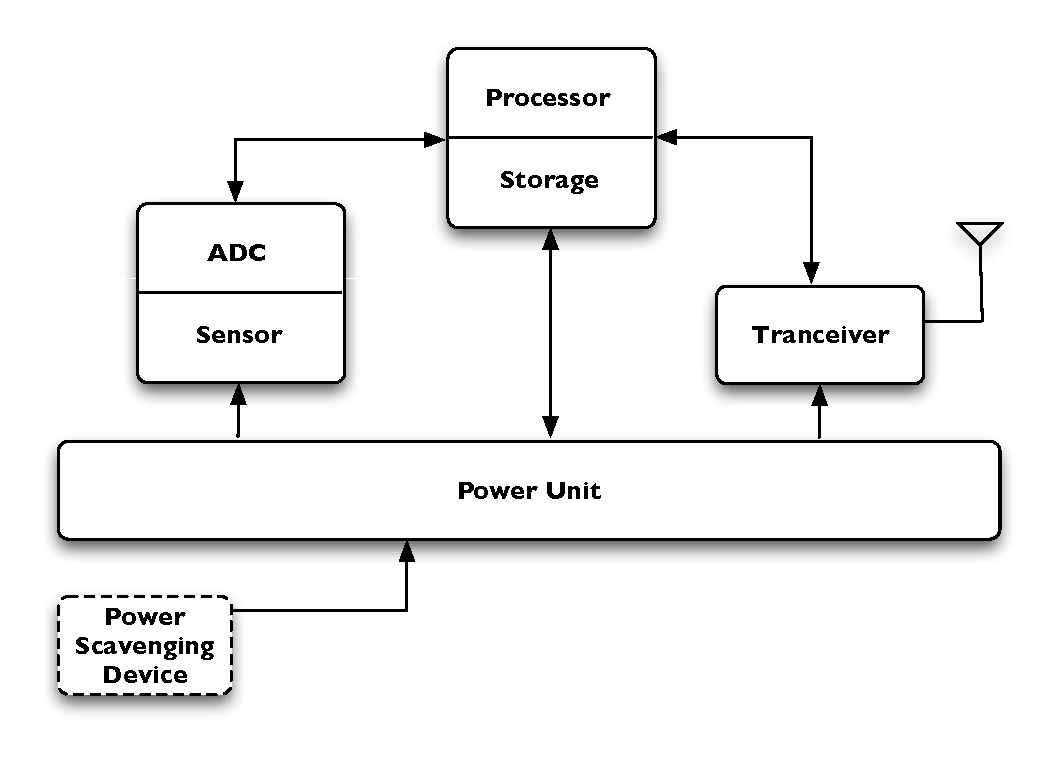
\includegraphics[scale=0.55]{img/SensorNodeArch.eps} \caption[Architecture of a 
sensor node] {Architecture of a sensor node (reproduced from
\cite{SensorSurveyAkyildiz:2002}). \emph{Note: The presence of components drawn using dotted lines is application dependent.}}
\end{figure} 

A typical sensor node is architected as follows 
\cite{SensorSurveyAkyildiz:2002}. It consists of a sensing unit, a processing 
unit, a transceiver unit, and a power unit as shown in Figure 
\ref{Fig:SensorNodeArch}.

The sensing unit is comprised of sensors and analog-to-digital converters. 
The sensors may either be built into the nodes, or be hot pluggable 
\cite{MANETWarrier:2007}. The processing unit usually comprises a 
microcontroller/microprocessor that performs processing, and is associated with 
a storage unit. The transceiver unit facilitates node-node communication using 
a variety of techniques. The power 
unit provides the energy required to run the sensor node, and can use chemical 
batteries or power scavenging units such as solar cells. This can be seen in 
Figure \ref{Fig:SensorNodeArch}.

Sensor nodes have constraints on both their size and their cost. The former 
constraint arises from the requirement that sensor nodes be easily deployable, 
while the latter arises from the requirement for fault tolerance (which in turn 
can be achieved only by being able to deploy cost-effectively large numbers of
sensor nodes in the environment being monitored). These limit the memory capacity, processing 
power, and the amount of energy available on a particular node.

\subsection{Wireless Sensor Networks}

As mentioned in the previous section, sensor nodes are capable of communicating 
untethered with one another, and are hence capable of forming networks of nodes 
called a Wireless Sensor Network. WSNs are typically deployed randomly in an
environment where phenomena are required to be monitored. A topology of a typical WSN has the 
following properties:

\begin{itemize}
\item A WSN is self-organising, given the random nature of the deployment.
\item The WSN topology is subject to change. Sensor nodes should be capable of 
dealing with changes of this kind in order to deal with hostile operating 
conditions, the failure-prone nature of sensor nodes and the possibility of 
redeployment of additional sensor nodes at any time during operation.
\end{itemize}

\section{WSN Protocol Stack} \label{sec:WSNProtStack}

The WSN protocol stack \cite{SensorSurveyAkyildiz:2002} is adapted from 
\cite{ComputerNetworksTannenbaum:2003}. While ignoring the division of the 
stack into planes as irrelevant to the understanding of the work presented 
herein, one may view the protocol stack as consisting of the following layers
(as can be seen from the Figure \ref{Fig:ProtStack}):

\begin{itemize}
\item \emph{Physical Layer:} This layer is responsible for the transmission of 
data over the physical transmission medium.
\item \emph{Data Link Layer:} This layer deals with power-aware Medium Access 
Control (MAC) protocols that minimise collisions and transceiver on-time.
\item \emph{Network Layer:} This layer is primarily responsible for routing  
data across the network.
\item \emph{Transport Layer:} ??? - DOES LN USE IT?
\item \emph{Application Layer:} This layer holds the application software.
\end{itemize}

The LN mechanism that forms the bedrock of this work (see 
Section \ref{LNDescription}) provides the functionality of the Data Link Layer 
and the Network Layer (CHECK WITH LUCA). The concept of Distributed Abstract
Data Types (see Section \ref{sec:DADT}) is restricted to the application layer,
and the focus of this work thus lies primarily within the application layer.

\begin{figure}
\centering
\label{Fig:ProtStack}
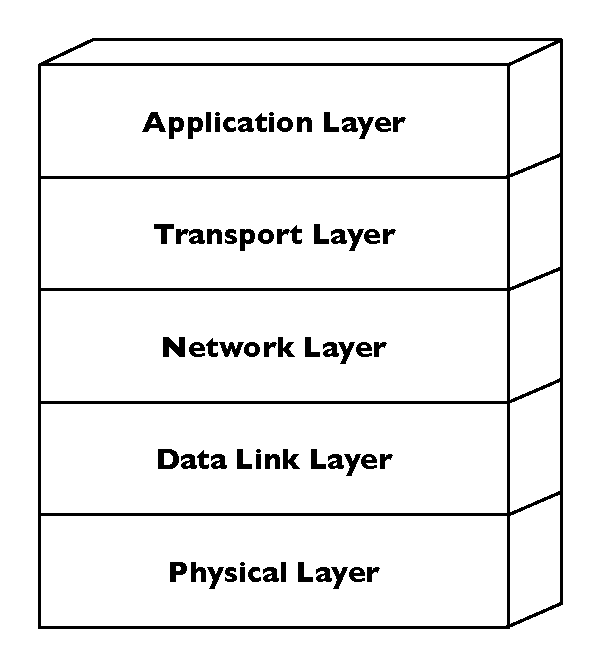
\includegraphics[scale=0.6]{img/ProtStack.eps}\caption[WSN protocol stack]{WSN protocol
stack (reproduced from \cite{SensorSurveyAkyildiz:2002})}
\end{figure}

\section {Programming models for WSNs}

\subsection{Motivation}
Current WSN programming paradigms are predominantly node-centric, wherein
applications are monolithic and tightly coupled with the protocols and algorithms
used in the lower layers of the protocol stack. The primary problem with this
approach is that most WSN applications are developed at an extremely low level of
abstraction, which requires the programmer to be knowledgeable in the field of
embedded systems programming. This stunts the growth in the use of WSNs in the
large space of application domains where it may be used
\cite{mottola_middleware:2008}.

 To increase the ubiquity of WSN
usage, it is essential that the protocols and mechanisms underlying WSN
development recede to the background, and the application programmer is
empowered to develop WSN applications at a higher level of abstraction. This
can be achieved using programming models which engineer a shift in focus
towards the system and its results, as opposed to sensor node functionality
itself \cite{mottola_middleware:2008}. 

\subsection{Benefits of using programming models}

According to Yu et al \cite{yu_issuesMiddleware:2004}, the use of such
programming models is beneficial for WSN applications because:
\begin{itemize}
\item The semantics of a WSN application can be separated from the details of 
the network communication protocol, OS implementation and hardware.
\item Efficient programming models may facilitate better utilisation of system 
resources.
\item They facilitate the reuse of WSN application code.
\item They provide support for the coordination of multiple WSN applications.
\end{itemize}

\subsection{Taxonomy of WSN Programming Models}

\begin{figure}
\centering
\label{Fig:ProgrammingModels}
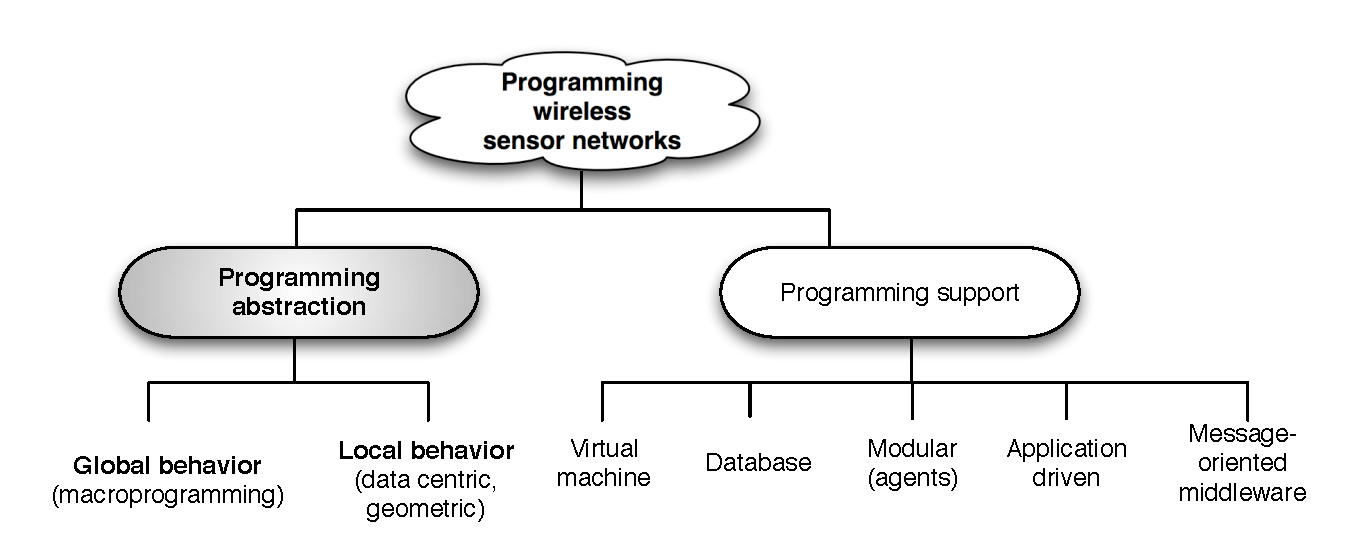
\includegraphics[scale=0.6]{img/ProgrammingAbstractions.eps} \caption[Taxonomy 
of WSN programming models]{Taxonomy of WSN programming models (reproduced from
\cite{hadim_middleware:2006})}
\end{figure}

Existing programming models for WSNs cover different areas and can serve 
different purposes. They can be classified into two main types, depending on 
the applications they are used for  \cite{hadim_middleware:2006} (see Figure
\ref{Fig:ProgrammingModels}):
\begin{itemize}
\item \emph{Programming support}, wherein services and mechanisms allowing for 
reliable code distribution, safe code execution, etc. are provided. Some
examples of programming models that take this approach include Mate
\cite{Levis_Mate:2002}, Cougar \cite{Bonnet_Cougar:2001}, SOS
\cite{Han_SOS:2005}, Agilla \cite{Fok_Agilla:2005}.
\item \emph{Programming abstractions}, where models deal with the global view 
of the WSN application as a system, and represent it through the concepts and 
abstractions of sensor nodes and sensor data. Some
examples of programming models that take this approach include Kairos
\cite{gummadi_Kairos:2005} and
EnviroTrack \cite{Abdelzaher_EnviroTrack:2004} .
\end{itemize}

The rest of this section focuses on the discussion of WSN programming
abstractions, as it is this type of programming model that is relevant to the
work presented herein.

\subsection{Classification of WSN Programming Abstractions}

\begin{figure}
\centering
\label{Fig:ProgrAbstrClassification}
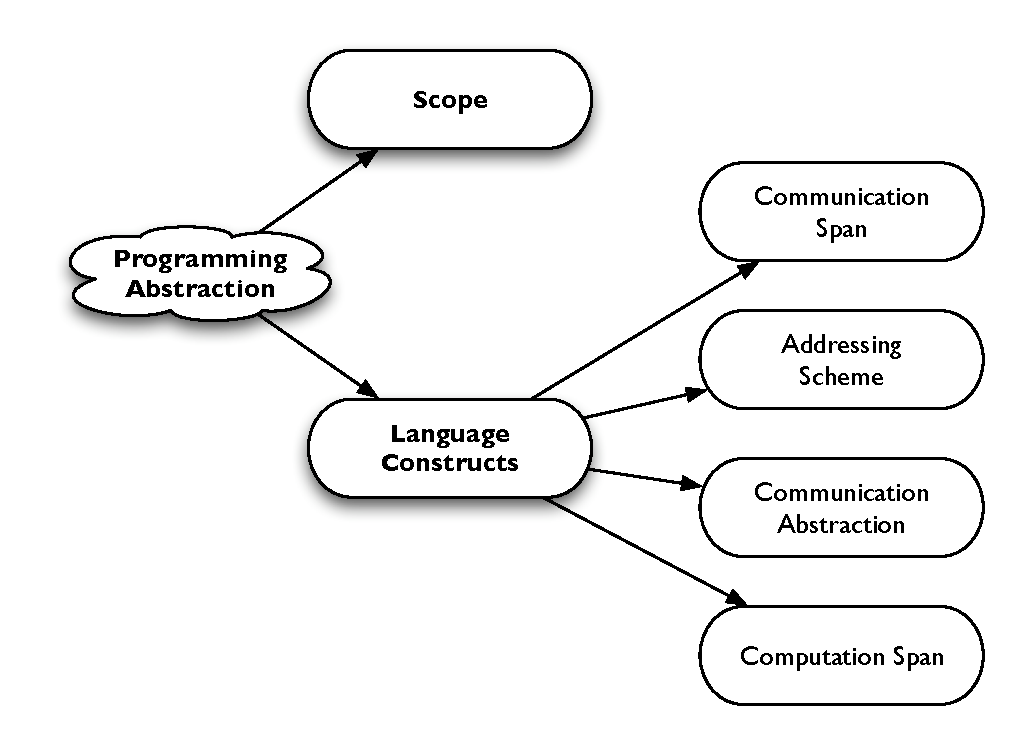
\includegraphics[scale=0.6]{img/ProgAbstr_Classification.eps}
\caption{Classification of Programming Abstractions} 
\end{figure} 

Programming abstractions may either be global (also referred to 
as macroprogramming) or local \cite{hadim_middleware:2006}. 

In the former case, the sensor network is programmed as a whole, and gets rid of
the notion of individual nodes \cite{mottola_middleware:2008}. Examples of
macroprogramming solutions include \emph{TinyDB} \cite{madden_TinyDB:2005} and
\emph{Kairos} \cite{gummadi_Kairos:2005}\footnote{N.B.: Kairos does not do away
with the notion of individual nodes as dedicated prorgramming constructs exist to
iterate through the neighbours of a given node}. 

In the latter case, the focus is on identifying relevant sections or
\emph{neighbourhoods} of the network. It is to be noted that these neighbourhoods
need not necessarily be physical. The framework used and developed during the
course of this work belongs to the latter class of programming abstractions.

Programming abstractions may also be classified on the basis of the
nature of the language constructs made available to the WSN programmer
\cite{mottola_middleware:2008}. Some of the metrics used for classification
are\footnote{Only relevant to this work classification bases, from among those
outlined in \cite{mottola_middleware:2008},were selected for discussion}:

\begin{itemize}
  \item Communication span
  \item Addressing scheme
  \item Communication abstraction
  \item Computation span
\end{itemize}

The rest of this section discusses each of these bases for classification in
detail, and is based on the work described in \cite{mottola_middleware:2008}
unless explicitly mentioned otherwise.

\subsubsection{Communication span}

The \emph{Communication span} enabled by a WSN programming interface is defined
as the set of nodes that communicate with one another in order to accomplish a
task. The communication span provided by a given abstraction can be:
\begin{itemize}
  \item \emph{Physical neighbourhood:} Abstractions using this approach provide
  the programmer with constructs to allow nodes to exchange data with others
  within direct communication range.
  \item \emph{Multi-hop group:} Abstractions that use this approach allow the
  programmer to exchange data among subsets of nodes in the WSN using
  multi-hop communication. These sets may either be
  \emph{connected}, wherein there always exists a path between any two nodes in
  the set, or \emph{non-connected/disconnected}.
  \item \emph{System-wide:} When using abstractions of this kind, the
  programmer can use constructs that allow data exchange between any two nodes
  of the entire WSN. This may be seen as an extreme manifestation of the
  \emph{Multi-hop group} approach described above.
\end{itemize}

\subsubsection{Addressing scheme}

The \emph{addressing scheme} specifies the mechanism by which nodes are
identified. Typically, there are two kinds of addressing schemes used:

\begin{itemize}
  \item \emph{Physical addressing:} Nodes are identified using statically
  assigned\footnote{S: not entirely convinced. Unique is better, methinks.}
  identifiers. The same address always identifies the same node (or nodes, if
  duplicate  identifiers exist) at any time during the execution of the
  application.
  \item \emph{Logical addressing:} Nodes are identified on the basis of
  predicates specified by the application programmer. Therefore, the same
  address (i.e., set of predicates) can identify different node(s) at different
  times.
\end{itemize}

\subsubsection{Communication Abstraction}

This classification basis defines the degree to which details of communication
in the WSN are hidden from the application programmer's view. Programming
interfaces may provide either:

\begin{itemize}
  \item \emph{Explicit communication} primitives where the
  programmer working in the application layer has to handle communication
  aspects such as buffering and parsing.
  \item \emph{Implicit communication}, where the programmer is unaware of the
  details of the communication process and performs communication using
  high-level constructs.
\end{itemize}

\subsubsection{Computation Span}

The \emph{Computation span} enabled by a WSN programming interface is defined
as the set of nodes that can be affected by the execution of a single
instruction. The
computation span provided by a given abstraction can be:

\begin{itemize}
  \item \emph{Node:} The effect of any instruction is restricted to a single
  node.
  \item \emph{Group:} Where the programmer is provided with constructs that
  could affect a subset of nodes.  
  \item \emph{Global:} An extreme case of previous type, a single instruction
  can impact every node in the WSN.
\end{itemize}

To illustrate, if it were possible in a given WSN programming abstraction to
send a \emph{Reset} message to all nodes with sensor readings greater than a
specific threshold, the computation span enabled is of type \emph{Group} (or
possibly \emph{Global}, which, as mentioned earlier, is an extreme case of the
\emph{Group} type).

\subsection{Programming models on the WSN protocol stack}

\begin{figure}
\centering
\label{Fig:ProtStack_ProgAbstr}
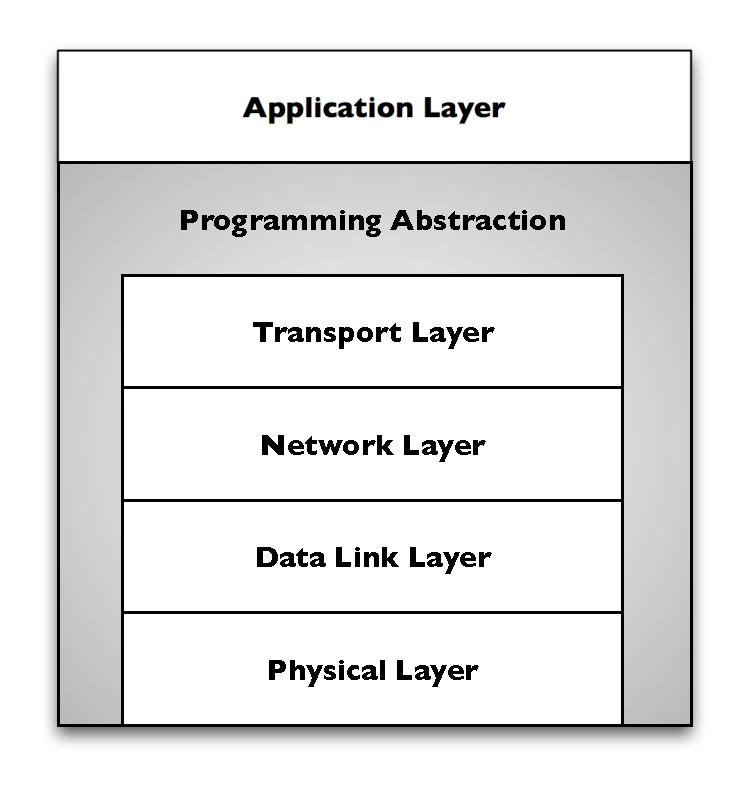
\includegraphics[scale=0.6]{img/ProtStack_ProgAbstr.eps}\caption[Programming
models on the WSN protocol stack]{Programming models on the WSN protocol
stack (adapted from \cite{mottola_middleware:2008})}
\end{figure}

WSN programming models are placed between the application layer and the
transport layer (change to network layer if trans layer not used) in the
protocol stack shown in Section \ref{sec:WSNProtStack}. As can be seen from
Figure \ref{Fig:ProtStack_ProgAbstr},
fine-grained details are hidden from the application programmer's view. The abstracted details
include:

\begin{itemize}
  \item Higher-layer services such as routing, localisation, and data storage
  mechanisms (and optimisations).
  \item Lower-layers such as the MAC protocol used, and the physical means of
  communication such as RF communication.
\end{itemize}


\section {Distributed Abstract Data Types} \label{sec:DADT}

Distributed Abstract Data Types is a new programming language construct used to
support distributed and context-aware applications. \cite{migliavacca_DADT:2006}
introduces the concept of DADTs, and presents a prototype that implements it.
The rest of this section discusses the concepts and the background, and
provides the reader with an understanding of the prototype.

N.B.: Every code snippet provided as an example is a code snippet based on the
DADT prototype described in \cite{migliavacca_DADT:2006}.

\subsection{Abstract Data Types}
An Abstract Data Type (ADT) is the representation of a model that presents an
abstract view to the problem at hand. The model of a problem defines:

\begin{itemize}
  \item The data affected.
  \item The operations identified.
\end{itemize}

This set of the data values and associated operations, independent of any
specific implementation, is called an ADT \cite{NIST_website}. 

One of the simplest example of an abstract data type is a stack, which
consists of the stacked data, and set of defined operations including \emph{push(Data), pop(),}
and \emph{top()}.

As is clear from the example, several different implementations of an ADT may
be defined from the proposed specification.

\subsubsection{ADTs in WSNs} \label{subsubsec:ADTsinWSN}

A WSN, as defined earlier, consists of several sensor nodes. Each sensor node
may include several sensors. By defining each sensor as
an ADT instance, the concept of ADTs can be used in WSNs. The code snippet below
shows the specification of a sensor ADT \ref{listing:ADTSpec}.   
  
\lstset{language = Java}  
 \begin{lstlisting}[frame=trbl, basewidth={0.55em, 0.6em}, captionpos=b, basicstyle=\ttfamily\footnotesize, breaklines, caption = Sensor ADT specification (reproduced from \cite{migliavacca_DADT:2006}), label = listing:ADTSpec ]
class Sensor {
  //data properties of the sensor 
    int sensorType;
    double[] sensorReading;
  //operations that can be performed on the sensor  
	public Sensor(type){
	  type = sensorType;
	  if (type == TEMPERATURE){
		sensorReading = new double[2];
	  }	else if (type == HUMIDITY){
		sensorReading = new double[1];
	  }
	}
    public double read(){ //read the sensor value(s).
	  ...
	} 
	public void reset(){ //reset the sensor
	  ...
	}
}
\end{lstlisting}

This specification declares that a Sensor ADT instance should provide the
following properties:
\begin{itemize}
\item An integer value to define the sensor type.   
\item An array of double values that holds the sensor reading. Depending on the
type of the sensor, the number of values read varies.
\end{itemize}

and the following operations:
\begin{itemize}
  \item A \emph{read} operation, that reads the sensor readings.
  \item A \emph{reset} operation, that resets it.
\end{itemize}

It is possible to define multiple such instances of this specification (for
example, the specification may be defined as a Java interface that has to
be implemented in order to create an ADT instance).

The ADT instances for a given sensor node that has two kinds of
sensors - (a) a temperature sensor, that senses the atmospheric and in-device
  temperature readings, and (b) A humidity sensor, that senses a single value -
  may be defined using the ADT specification described above as shown in
  Listing \ref{listing:ADTInstances}. This is quite similar to the declaration
  of the object of a class.  

\begin{lstlisting}[frame=trbl, basewidth={0.55em, 0.6em}, captionpos=b,
basicstyle=\ttfamily\footnotesize, breaklines, caption = Sensor ADT instances, label =
listing:ADTInstance ]
  // Temperature sensor ADT instance
  Sensor temperatureSensor = new Sensor(TEMPERATURE);
  ...
  // Humidity sensor ADT instance  
  Sensor humiditySensor = new Sensor(HUMIDITY);
\end{lstlisting}

Thus, multiple ADTs can be used to abstract the nature of the
sensor node, as well as the sensors therein, from the programmer. 

\subsubsection{Data and space ADTs} \label{subsubsec:DataAndSpaceADTs}

As a WSN consists of a collection of sensor nodes that are distributed in
space, ADTs can also be used to describe the spatial location of a given
sensor node. Thus, ADTs used in WSNs are of two types:

\begin{itemize}
  \item \emph{Data ADTs} are ``conventional'' ADTs which encode
  application logic (for example, allowing access to sensor data).
  \item \emph{Space ADTs}, also known as \emph{sites}, are ADTs that provide an
  abstraction of the computational environment (in the case of a WSN, a sensor
  node) that ``hosts the data ADT'' \cite{migliavacca_DADT:2006}. The space ADT
  may use different notions of space, such as physical location or netwo
 rk topology, depending on application requirements as determined by the
 programmer. A very limited notion of space is built into the DADT prototype in
 \cite{migliavacca_DADT:2006}, by means of a superclass called \emph{Site} which
 every Space ADT specification inherits from.
\end{itemize}

The ADTs presented in the previous section are examples of data ADTs. Space
ADTs are defined and implemented in a similar manner, except for changes in
their properties and operations (see Listing \ref{listing:SpaceADTSpec} for the
specification of a Space ADT).  
 
 \begin{lstlisting}[frame=trbl, basewidth={0.55em, 0.6em}, captionpos=b, basicstyle=\ttfamily\footnotesize, breaklines, caption = Sensor Space ADT specification (reproduced from \cite{migliavacca_DADT:2006}), label = listing:SpaceADTSpec ]
class SensorLoc extends Site {
  //space properties of the sensor 
	location l;
  //operations that can be performed on the sensor
	public SensorLoc(Location l){
	  this.l = l;
	}
	public double[] getLocation(){ //read the sensor value(s).
	  ...
	}
	public void getBatteryLevel(){ //reset the sensor
	  ...
	}
}
\end{lstlisting}
 
\subsubsection{Placement}
 
As described in Section \ref{subsubsec:DataAndSpaceADTs}, a space ADT defines
the computing environment that ``hosts'' the data ADT. A data ADT can be
associated with the corresponding space ADT using a placement operation\footnote{the placement operation is
performed explicitly by the application programmer.} as can be seen in Figure \ref{Fig:DADTs}.
A Sensor data ADT
instance can be ``placed'' in a SensorLoc space ADT instance as shown in Listing
\ref{listing:placement}. 

\begin{lstlisting}[frame=trbl, basewidth={0.55em, 0.6em}, captionpos=b, basicstyle=\ttfamily\footnotesize, breaklines, caption = ADT placement, label = listing:placement ]
  tempSensor = new Sensor(TEMPERATURE);
  sensorLoc = new SensorLoc(sensorGPSLocation);
  
  place(tempSensor, sensorLoc)
\end{lstlisting}

\subsection{DADTs as an extension of ADTs}
An extension of ADTs - a class of Distributed ADTs (DADTs), have applications 
in distributed programming models. The state of multiple ADTs in a distributed
system are made collectively available using the interface of a DADT
\cite{migliavacca_DADT:2006}. 

Using properties that are applied over multiple ADT instances, DADTs can be
used to define views over the distributed state. Views allow for the dynamic
restriction of the scope of distributed operations that the application
requires to perform. 

They can be used when the distributed state 
of the system is the primary issue of importance. Similar to ADTs, DADTs 
provide specifications for distributed data, distributed operators, and 
constraints.

The notion of space is extended to DADTs, and therefore DADTs can either be:

\begin{itemize}
  \item \emph{Space DADT:} allows distributed access to a collection of space
  ADTs. 
  \item \emph{Data DADT:} allows distributed access to a collection of data ADTs.
\end{itemize}

The rest of this section presents the use of DADTs, specifically in relation to
the DADT prototype \cite{migliavacca_DADT:2006}.

\subsubsection{DADT specification and instantiation} \label{subsubsec:dadtspecandinst}

DADT specifications can be best understood by carrying forward the example
described in Section \ref{subsubsec:ADTsinWSN}. To allow for collective access
to multiple ADT instances of the type specified in Listing
\ref{listing:ADTSpec}, a DADT \emph{DSensor} may be defined as shown in Listing
\ref{listing:DADTSpec}.   
 
\begin{lstlisting}[frame=trbl, basewidth={0.55em, 0.6em}, captionpos=b, 
basicstyle=\ttfamily\footnotesize, breaklines, caption = Data DADT 
specification (reproduced from \cite{migliavacca_DADT:2006}), label = 
listing:DADTSpec]
datatype DSensor distributes Sensor with {
  operations:
	void resetAll();
	double average();
}
\end{lstlisting}

The DADT specification allows two operations to be performed on multiple data 
ADTs of type Sensor:  
\begin{itemize}
\item \emph{resetAll():} Resets every sensor in the DADT view.
\item \emph{average():} Calculate the average of readings of every sensor in the
view.
\end{itemize}

DADT specifications can be instantiated as an object of a class would, and can
be used to perform distributed operations (see Listing \ref{listing:DADTInstance}).

\begin{lstlisting}[frame=trbl, basewidth={0.55em, 0.6em}, captionpos=b, 
basicstyle=\ttfamily\footnotesize, breaklines, caption = DADT Instantiation 
(reproduced from \cite{migliavacca_DADT:2006}), label = listing:DADTInstance ]
DSensor ds = new DSensor();
double v = ds.average();
\end{lstlisting}

As can be seen from this listing, the distributed nature of the DADT can be
abstracted from the application programmer.

\subsubsection{Binding}

The set of ADTs that are available for collective access using a DADT (in this
case, the collection of ADTs of type Sensor) is called the \emph{member set} of
the DADT.

An ADT instance is made part of the member set by binding it to the DADT type. This is done using a dedicated
programming construct as shown in Listing \ref{listing:binding}, where the
Sensor ADT (see Listing \ref{listing:ADTSpec}) is bound to the DADT type \emph{DSensor}
defined in Listing \ref{listing:DADTInstance}. 
 
 
\begin{lstlisting}[frame=trbl, basewidth={0.55em, 0.6em}, captionpos=b, 
basicstyle=\ttfamily\footnotesize, breaklines, caption = Binding ADT instances to a DADT instance, label = listing:binding ]
bind(new Sensor(TEMPERATURE), ``DSensor");
...
bind(new Sensor(HUMIDITY), ``DSensor");
\end{lstlisting} 
 

\subsubsection{Operators and Actions} \label{subsubsec:OperatorsAndActions}

Operators are used to allow distributed access and operations to be performed on
ADT instances bound to a given DADT type. Operators are executed on the DADT
instance, and may be of the following types:

\begin{itemize}
  \item \emph{Selection Operators:} Selection operators allow for an operation
  to be performed on a subset of the instances in the member set.
  \item \emph{Conditional Operators:} Conditional operators make the code in the
  DADT method dependent on a global condition on the member set. 
  \item \emph{Iteration Operators:} These operators allow iterating over the ADT
  instances in the target set, and thus permit access to individual ADT instances.
\end{itemize}

Actions are constructs defined in the DADT type that causes the execution of an
operation on a remote ADT instance. This can be understood by looking at the
following example.

To perform a DADT read operation, an action is defined
as shown in Listing
\ref{listing:DADTAction}. 
 
\begin{lstlisting}[frame=trbl, basewidth={0.55em, 0.6em}, captionpos=b, 
basicstyle=\ttfamily\footnotesize, breaklines, caption = Defining a DADT action, label = listing:DADTAction ]  
public class DSensor_read_Action implements DADT.Action{

  public Object evaluate(Object ADTInstance){
	Sensor localSensor = (Sensor) ADTInstance;
    return localSensor.read();
  }
}
\end{lstlisting}

This performs the operation on the ADT Instance of type \emph{Sensor} (see
Listing \ref{listing:ADTSpec}).

When the application programmer attempts to execute a DADT operation, such as
for instance, the computation of the average
across all sensors in its target set (see Listing \ref{listing:DADTInstance}),
actions of the sort defined above are called\footnote{The details of the
implementation of actions are outlined in Chapter \ref{chap:Implementation}.} 

\subsubsection{Views} \label{subsubsec:views}

The concept of views is summarised in Figure \ref{Fig:DADT_Views}.

A \emph{property} is a DADT characteristic that is defined in terms of an ADT's
data and operations, and is executed locally on the ADT instance
\cite{migliavacca_DADT:2006}. Properties work on a principle similar to that of
actions (see Section \ref{subsubsec:OperatorsAndActions}).

The member set may be partitioned into \emph{DADT views} using properties. A
DADT view may either be a (1) space view or a (2) data view. In the rest of this
section, we focus on data views as space views are irrelevant to the
understanding of this work. 

To continue on the example running throughout this section, If the application
programmer wished to partition the set of sensors bound to the DADT type
\emph{DSensor} in Listing \ref{listing:binding} to refer to only those ADT
instances that are temperature sensors, a Data View is defined as shown in Listing
\ref{listing:views} 
  
\begin{lstlisting}[frame=trbl, basewidth={0.55em, 0.6em}, captionpos=b, 
basicstyle=\ttfamily\footnotesize, breaklines, caption = Definition and use of DADT Data View, label = listing:views ]  
DataView dv = new DataView(new DSensor_typeOf_Property(TEMPERATURE));

double[] averageTemperatures = ds.average(dv);
\end{lstlisting}

The data view \emph{dv} specifies that the scope of the DADT operation
\emph{average} is restricted to temperature sensors.

\begin{figure}
\centering
\label{Fig:DADTs}
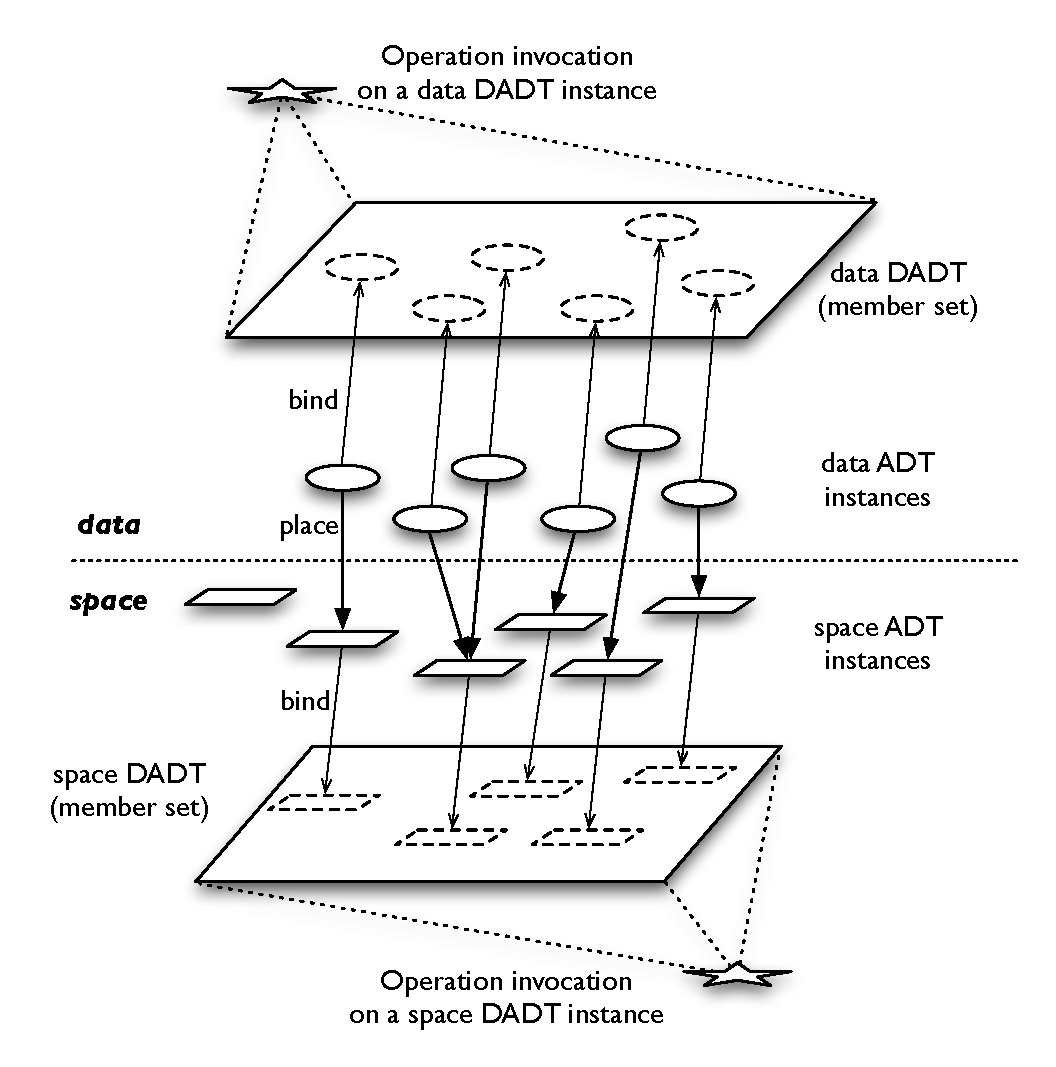
\includegraphics[scale=0.50]{img/DADTs.eps} \caption[Data and space in the DADT 
model]{Data and space in the DADT model (reproduced from 
\cite{migliavacca_DADT:2006})}
\end{figure}

\begin{figure}
\centering
\label{Fig:DADT_Views}
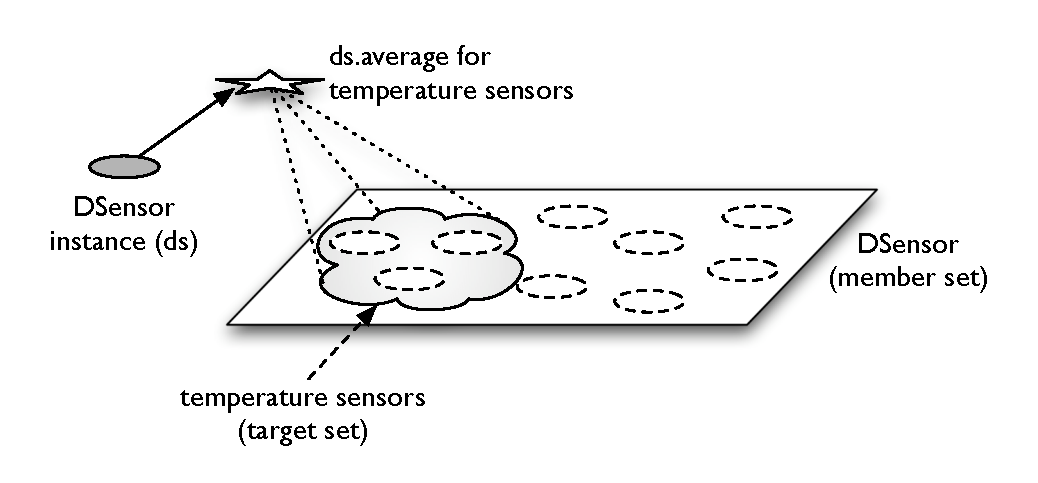
\includegraphics[scale=0.50]{img/DADT_Views.eps} \caption[DADT views]{DADT views
(reproduced from 
\cite{migliavacca_DADT:2006})}
\end{figure}

\subsection {DADT prototype limitations}

The prototype presented in \cite{migliavacca_DADT:2006} was developed as a proof of 
concept. The prototype uses IP multicast to simulate the lower layers of the 
protocol stack, thereby preventing its use in simulators or real nodes. This 
work sets out to correct this limitation by combining the DADT prototype with 
an implementation of logical neighborhoods. %?????Additionally, the full
%??? ASK functionality of  space DADTs has not been implemented in the
%??? prototype.

\section {Logical neighbourhoods} \label{LNDescription}

Typically, communication between WSN nodes is based on routing 
information between nodes by exploiting the communication radius of each node.
Thus, the notion of a node's physical neighbourhood - the set of nodes in the
network
that fall within the communication range of a given node - is central to this.

However, in heterogenous WSN applications, the developer might require to
communicate with a specific subset of the network that is defined logically and
not physically. As an example of this, consider the following example. An
application that provides security in a high-risk environment by monitoring 
motion might require - in the event of a security alarm - all sensors at the
entrances to the guarded area to report a recent history of recorded motion.
The sensors at the entrance form a logical neighbourhood in this case. However,
as the entrances may be widely separated, it is not necessary that this subset
of nodes is part of a single physical neighbourhood. The use of current WSN
programming techniques to enable a mechanism of this nature entails additional
programming effort, increased complexity, and less reliable code
\cite{mottola_LN:2006}.  

\begin{figure} 
\centering
\label{Fig:LN_physical_vs_logical}
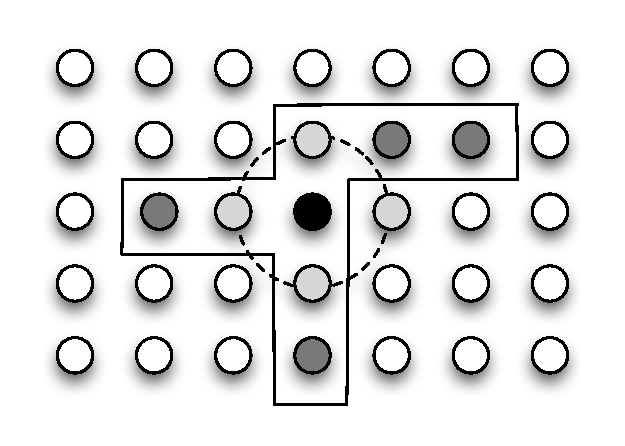
\includegraphics[scale=0.65]{img/LN_physical_vs_logical.eps} 
\caption[Difference between physical and logical neighborhoods]{Representation 
of logical and physical neighborhood of a given node. \emph{The dashed circle 
represents the physical neighborhood, whereas the solid polygon represents (one 
of) the node's logical neighborhood} (reproduced from
\cite{mottola_LN:2006})}
\end{figure} 

Mottola and Picco \cite{mottola_LN:2006} suggest the addressing of the
aforementioned issues by using \emph{Logical Neighbourhoods (LNs)}, an abstraction
that replaces the node's physical neighbourhood with a logical notion of
proximity (See example above, and Figure \ref{Fig:LN_physical_vs_logical}). Using this abstraction, programmers
can communicate
with members of a LN using a simple message passing API,
thereby allowing for logical broadcasts. The implementation of the aforementioned API is
supported by means of a novel routing mechanism devised specifically to support
LN communication.

The rest of this section discusses the LN abstraction and the
underlying routing mechanism in greater detail.

\subsection{The LN Abstraction}

\subsubsection{Specification}

LNs can be specified using a declarative language such as SPIDEY
\cite{mottola_LN:2006, mottola_LNScoping:2006}\footnote{The LN prototype used as
part of this work does not use a declarative language for LN specification}, and
involves the definition and instantiation of the \emph{node} and the
\emph{neighbourhood}. 

Nodes are a logical representation of the subset of a sensor node's state and
characterstics that are used for the specification of an LN. Nodes are defined
in a \emph{node template} and are subsequently instantiated, as shown in Listing \ref{listing:LN1}
   
\begin{lstlisting}[frame=trbl, basewidth={0.55em, 0.6em}, captionpos=b, 
basicstyle=\ttfamily\footnotesize, breaklines, caption = Node Definition and Instantiation, label = listing:LN1 ]  
node template Sensor
  static Function
  static Type
  dynamic BatteryPower
  dynamic Reading

create node ts from Sensor
  Function as ``Sensor''
  Type as ``Temperature''
  Reading as getTempReading()
  BatteryPower as getBatteryPower()
\end{lstlisting}

A neighbourhood can be defined by applying predicates on the attributes defined
in the
node template. The neighbourhood is defined using a neighbourhood
template, and subsequently instantiated. 

Listing \ref{Listing:LN2} shows the definition and
instantiation of a
neighbourhood - based on the node template defined in Listing \ref{Listing:LN1}
- which selects all temperature sensors where the reading exceeds a threshold.
 
\begin{lstlisting}[frame=trbl, basewidth={0.55em, 0.6em}, captionpos=b, 
basicstyle=\ttfamily\footnotesize, breaklines, caption = Neighbourhood Definition and Instantiation, label = listing:LN2 ]  
neighbourhood template HighTempSensors(threshold)
  with Function = ``Sensor'' and Type  = ``Temperature'' and Reading > Threshold

create neighbourhood HigherTemperatureSensors
  from HighTempSensors(threshold:45)
\end{lstlisting}

\subsubsection{Communication}

Communication using LNs is performed using a simple API which overrides the
traditionally used broadcast facility and makes it dependent on the (logical)
neighbourhood the message is addressed to \cite{mottola_LN:2006}. The routing mechanism described in
the next section enables LN commmunication.

\subsection{Routing}

The routing approach used in LNs is structure-less, and uses a local search
mechanism based on a distributed state space built by the periodic updation of
node profiles. The routing mechanism can be divided into two phases \cite{mottola_LNAbstraction}:

\subsubsection{Phase 1: Construction of a distributed state space}
Each node periodically transmits a \emph{profile advertisement} that contains
information on the attribute-value pairs defined in the node template. This message
causes an
update in its physical neighbours' \emph{State Space Descriptors (SSDs)} if (a)
no
entry exists for any given attribute-value pair specified in the profile
advertisement, or (b) the \emph{transmit cost} is lower than the costs for any
existing SSD entry for a particular attribute-value pair. If any such change
occurs, the profile advertisement is rebroadcast with an updated cost. 

Additionally, passive listening to profile advertisements for attribute-value
pairs with higher costs than what is entered in the SDD is used to construct
increasing paths.

\subsubsection{Phase 2: Routing through Local Search}
When a message has to be sent to a particular LN, the sending node sends the
message to any node in its SSD whose attribute-value pairs match the LN
predicates. The message is associated with a specific set of \emph{credits} from
which the cost to send to the node is deducted. This process continues until the
message is received at node(s) in the LN along the reverse of the path
determined during the first phase. This path is called a \emph{decreasing path}.

However, to ensure that messages are received by every nodes that belongs to the
neighbourhood (and the algorithm is not trapped in local state-space minima),
\emph{exploring paths} are used at specific points during the message traversal
(at nodes which meet the neighbourhood predicates, and/or after a user-defined
number of hops). The credit reservation system described above is used in that
case, with the node dividing the reserved credits between following decreasing
paths and exploring paths.

\section {JiST/SWANS} \label{sec:jistswans}

As the simulator used in this work is a discrete event simulator, this section 
begins with a short description of discrete event simulators. 
This is followed by a discussion on a particular discrete event simulator
called JiST, and the SWANS network simulator built on top of JiST.

\subsection{Discrete Event Simulator}

A discrete event simulator allows for the simulated execution of a process (that
may be either deterministic or stochastic), and consists of the following
components \cite{Shankar_DiscreteEventSim}:

\begin{itemize}
  \item \emph{Simulation variables:} These variables keep track of simulation 
  time, the list of events to be simulated, the (evolving) system state, and 
  performance indicators.
  \item \emph{Event handler:} The event handler schedules events for execution 
  at specific points in simulation time (and unschedules them if necessary), 
  and additionally updates the state variables and performance indicators.
\end{itemize}
 
\subsection{Java In Simulation Time (JiST)} \label{subsec:jist}

JiST \cite{barr_JIST:2005} is a discrete event simulator that is 
efficient (compared to existing simulation systems), 
transparent (simulations are automatically translated to run with the 
simulation time semantics), and standard (simulations use a
conventional programming language, i.e., Java).

JiST simulation code is written in Java, and converted to run over the JiST 
simulation kernel using a bytecode-level rewriter\footnote{N.B.: The bytecode 
rewriter and the simulation kernel are both written in Java},  as can be seen 
in Figure \ref{Fig:JiST_architecture}.

The execution of a JiST program can be understood by considering example as
shown in Listing \ref{listing:JiSTExample}

\begin{lstlisting}[frame=trbl, basewidth={0.55em, 0.6em}, captionpos=b, 
basicstyle=\ttfamily\footnotesize, breaklines, caption = Example JiST program (reproduced from \cite{barr_JIST:2005}, label = listing:JiSTExample]  
import jist.runtime.JistAPI;  
class hello implements JistAPI.Entity { 
  public static void main(String[] args) { 
    System.out.println("Simulation start"); 
    hello h = new hello(); 
    h.myEvent(); 
  } 
  public void myEvent() { 
    JistAPI.sleep(1); 
    myEvent(); 
    System.out.println("hello world, " + JistAPI.getTime()); 
  }} 
\end{lstlisting}

\begin{figure}
\centering
\label{Fig:JiST_architecture}
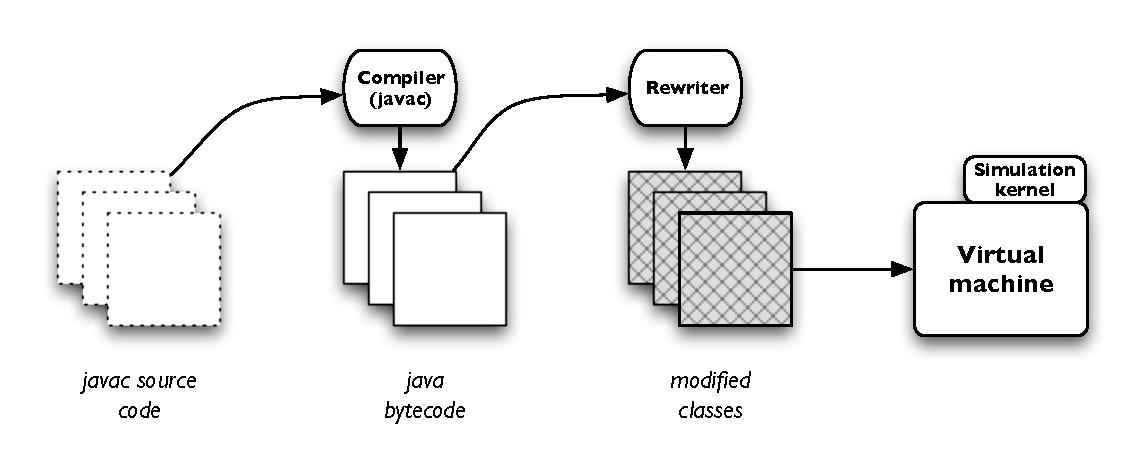
\includegraphics[scale=0.72]{img/JiST_architecture.eps} \caption[The JiST 
System Architecture]{The JiST system architecture (reproduced from
\cite{barr_JIST:2005})}
\end{figure}  
 
This program is then compiled and executed in the JiST simulation
kernel, using the following commands:

  
\begin{lstlisting}[frame=trbl, basewidth={0.55em, 0.6em}, captionpos=b, 
basicstyle=\ttfamily\footnotesize, breaklines, caption = Execution of the
program in the JiST, label = listing:JiST ]  
javac hello.java
java jist.runtime.Main hello
\end{lstlisting}


The simulation kernel is loaded upon execution of this command. This kernel
installs into the JVM a class loader that performs the rewrite of the bytecode.
The JistAPI functions used in the example code are used to perform the
code transformations. The method call to myEvent is now scheduled and executed
by the simulator in simulation time. Simulation time differs from ``actual''
time in that the advancement of actual time is independent of application
execution. 
 
\subsection{Scalable Wireless Ad hoc Network Simulator (SWANS)}
SWANS is a wireless network simulator developed in order to provide efficient
and scalable simulations without compromising on simulation detail \cite{barr_SWANS},
and is built upon the JiST discrete event simulator described in Section \ref{subsec:jist}. 
It is organised a a collection of independent, relatively simple, event driven
components that are encapsulated as JiST entities. 
  
SWANS has the following capabilities \cite{barr_SWANS}:

\begin{itemize}
\item The use of
interchangeable components enables the construction of a protocol stack for the
network, and facilitates parallelism, and execution in a distributed environment.
\item Can execute unmodified Java network applications on the
simulated network (in simulation time), by virtue of its being built over
JiST.Using a harness, the aforementioned Java code is automatically rewritten to
run on the simulated network.  
\end{itemize}
   
The SWANS architecture may be seen in Figure \ref{Fig:SWANS_architecture}. 

\begin{figure}[ht]
\centering
\label{Fig:SWANS_architecture}
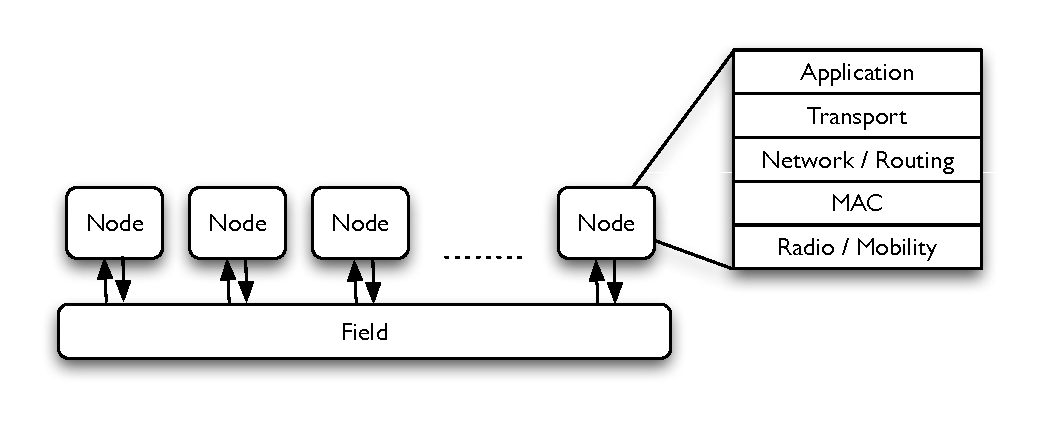
\includegraphics[scale=0.71]{img/SWANS_architecture.eps} \caption[SWANS 
architecture]{SWANS architecture}
\end{figure} 

\section {Sun SPOTs} \label{sec:sunspots}

\subsection{Motivation}

Sensor nodes, as mentioned in Section \ref{subsec:sensornodes}, are
characterised by limited resources, including memory.
 
Managed runtime languages like Java were not used for sensor network programming
because of the combination of the static memory footprint of the Java Virtual
Machine (JVM) and the dynamic memory footprint of the WSN application code.

In order to overcome
memory limitations, wireless sensor network applications have traditionally been
 coded in non-managed languages like C and assembly language
 \cite{simon_squawk:2006}. 
 
 On the other hand, it is widely accepted that development times are greatly reduced
upon the use of managed runtime languages such as Java
\cite{simon_squawk:2006}. Therefore, currently prevalent WSN programming practice
trades developer efficiency for memory efficiency. 

However, Simon et al \cite{simon_squawk:2006} state the benefits accrued from
using a managed runtime language for WSN programming as follows:

\begin{itemize}
  \item Simplification of the process of WSN programming, that would cause an
  increase in developer adoption rates, as well as developer productivity.
  \item Opportunity to use standard development and debugging tools.
\end{itemize}
 
\subsection{The Sun SPOT hardware platform }
Sun Microsystems has, on the basis of the arguments discussed in the previous
section, built a sensor device
called the Sun Small Programmable Object Technology (Sun SPOT) that uses a
on-board JVM to allow for WSN programming using Java.

The Sun SPOT uses an ARM-9 processor, has 512 KB of RAM and 4 MB of flash
memory, uses a Chipcon CC 2420 IEEE 802.15.4 compliant radio to enable
wireless RF communication between nodes, and allows for pluggable sensors.

\subsection{The Squawk JVM}

The Squawk JVM is used on Sun SPOTs to enable on-board execution of Java
programs. The Squawk VM was originally developed for a smart card system with
even greater memory constraints than the Sun SPOTs. The Squawk JVM has the
following features \cite{simon_squawk:2006}:

\begin{itemize}
  \item It is written in Java, and specifically designed for resource
  constrained devices, meeting the Connected Limited Device Configuration
  (CLDC) Java Micro Edition (Java ME) configuration requirements.
  \item It does not require an underlying OS, as it runs directly on the Sun
  SPOT hardware. This reduces memory consumption.
  \item It allows for inter-device application migration.
  \item It authenticates deployed applications.
  \item It supports the execution of multiple applications on one VM,
  representing each one as an object.
\end{itemize}

\subsection{Split VM Architecture}

As resource constrained devices are incapable of loading class files on-device
by virtue of their limited memory, a VM architecture known as the ``split VM
architecture'' is used (See Figure \ref{Fig:SquawkVM_architecture}. 

The Squawk split VM architecture uses a class file preprocessor (known as the
suite creator) that converts the \emph{.class} bytecode into a more compact
representation called the Squawk bytecode. According to
\cite{simon_squawk:2006}, Squawk bytecodes are optimised in order to:
\begin{itemize}
\item minimise space used by using smaller bytecode representation, escape
mechanisms for float and double instructions, and widened operands. 
\item allow for in-place execution, by ``resolving symbolic references to other
classes, data members, and member functions into direct pointers, object offsets
and method table offsets respectively'' \cite{simon_squawk:2006}.
\item simplify garbage collection, by the careful reallocation of local
variables and storing on the operand stack only the operands for those
instructions that would result in a memory allocation.
\end{itemize}

The Squawk bytecodes are converted into a \emph{.suite} file created by
serialising and saving into a file the internal object memory representation.
These files are loaded on to the device, and subsequently interpreted by the
on-device VM.
  
\begin{figure}
\centering
\label{Fig:SquawkVM_architecture}
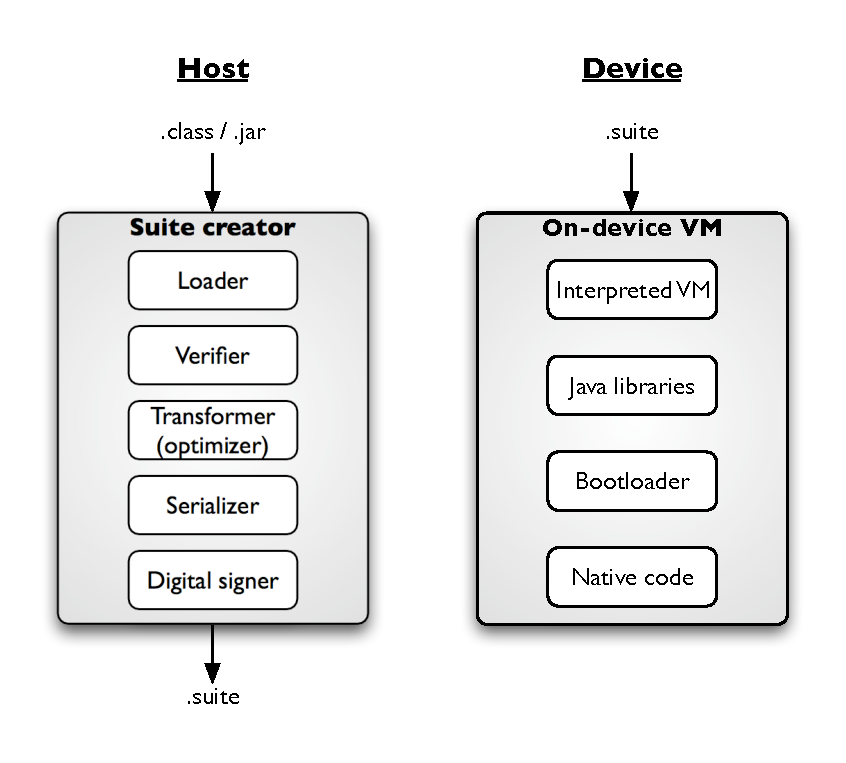
\includegraphics[scale=0.71]{img/Squawk_architecture.eps} \caption[The Squawk
Split VM Architecture]{The Squawk
Split VM Architecture (reproduced from \cite{simon_squawk:2006})}
\end{figure}   
  

